% Template for solutions write-ups, STAT 460/560
% Some basic notation is defined in 'macros/basic-math-macros'

\documentclass{article}
\usepackage{verbatim}
\usepackage{titlesec}

\def\coursename{STAT 447C: Bayesian Statistics}
\def\semester{Fall 2024}

\setlength{\oddsidemargin}{0.0 in}
\setlength{\evensidemargin}{0.0 in} 
\setlength{\topmargin}{-0.6 in} 
\setlength{\textwidth}{6.5 in} 
\setlength{\textheight}{8.5 in}
\setlength{\headsep}{0.75 in} 
\setlength{\parindent}{0 in}
\setlength{\parskip}{0.1 in}

\titleformat*{\section}{\Large\bfseries}


% prints box at top of first page with relevant info
\newcommand{\problemset}[3]{
   \pagestyle{myheadings}
   \thispagestyle{plain}
   \newpage
   \noindent
   \begin{center}
   \framebox{
      \vbox{\vspace{2mm}
    \hbox to 6.28in { {\bf \coursename
                        \hfill \semester} }
       \vspace{4mm}
       \hbox to 6.28in { {\Large \hfill #3  \hfill} }
       \vspace{2mm}
       \hbox to 6.28in { {\it #1 \hfill \texttt{#2}} }
      \vspace{2mm}}
   }
   \end{center}
   \vspace*{4mm}
}

\newcommand{\qsol}[1]{\section{#1}}
  % DO NOT CHANGE
% \usepackage{graphicx,amssymb,amsmath,amsthm,mathrsfs}
% \usepackage{multirow,makeidx,algorithmic,algorithm}
\usepackage{multirow,makeidx,algpseudocode,algorithm}
\usepackage{mathtools}
\usepackage{enumitem}
 
\usepackage{parskip}
\usepackage{setspace}
\usepackage{float, graphicx}
\usepackage{adjustbox}
\usepackage{bbm}
\usepackage{tabularx}
\usepackage{subfigure}
\usepackage{amsmath,amssymb,amsfonts,amsthm,amsbsy,amstext,mathrsfs}
\usepackage{hyperref}
\usepackage{url}
\usepackage{color}
\usepackage{graphicx} % Required for inserting images
\usepackage[utf8]{inputenc}

%% reference
\usepackage[round]{natbib}
\bibliographystyle{abbrvnat}
% \usepackage{cite}
% \bibliographystyle{plainurl}
% \bibliographystyle{abbrv}
% \bibliographystyle{plain}
% \bibliographystyle{unsrt}


%% code in-text
\usepackage{listings}
\usepackage{xcolor}

\definecolor{codegreen}{rgb}{0,0.6,0}
\definecolor{codegray}{rgb}{0.5,0.5,0.5}
\definecolor{codepurple}{rgb}{0.58,0,0.82}
\definecolor{backcolour}{rgb}{0.95,0.95,0.92}

\lstdefinestyle{mystyle}{
    backgroundcolor=\color{backcolour},   
    commentstyle=\color{codegreen},
    keywordstyle=\color{magenta},
    numberstyle=\tiny\color{codegray},
    stringstyle=\color{codepurple},
    basicstyle=\ttfamily\footnotesize,
    breakatwhitespace=false,         
    breaklines=true,                 
    captionpos=b,                    
    keepspaces=true,                 
    numbers=left,                    
    numbersep=5pt,                  
    showspaces=false,                
    showstringspaces=false,
    showtabs=false,                  
    tabsize=2
}

\lstset{style=mystyle}


%% layout
\oddsidemargin 3mm
\evensidemargin 3mm
\topmargin -12mm
\textheight 660pt
\textwidth 450pt  % DO NOT CHANGE
% ADD YOUR CUSTOM NOTATION HERE
\newcommand{\R}{\mathbb R}
\newcommand{\Z}{\mathbb Z}
\newcommand{\Q}{\mathbb Q}
\newcommand{\N}{\mathbb N}
\newcommand{\C}{\mathbb{C}}
\newcommand{\1}{\mathbbm{1}}
\newcommand{\E}{\mathbb E}
\newcommand{\Mcal}{{\cal M}}
\newcommand{\Ncal}{{\cal N}}
\newcommand{\Acal}{{\cal A}}
\newcommand{\Bcal}{{\cal B}}
\newcommand{\Fcal}{{\cal F}}
\newcommand{\Ecal}{{\cal E}}
\newcommand{\Gcal}{{\cal G}}
\newcommand{\Hcal}{{\cal H}}
\newcommand{\Scal}{{\cal S}}
\newcommand{\Xcal}{{\cal X}}
\newcommand{\Lcal}{{\cal L}}
\newcommand{\Mscr}{\mathscr{M}}
\newcommand{\eps}{\varepsilon}
\renewcommand{\P}{\mathbb P}
\DeclareMathOperator{\Var}{Var}
\DeclareMathOperator{\Poi}{Poi}
\DeclareMathOperator{\Cov}{Cov}
\DeclareMathOperator{\Exp}{Exp}
\DeclareMathOperator{\Bin}{Bin}
\DeclareMathOperator{\Geom}{Geom}
\DeclareMathOperator{\Unif}{Unif}
\DeclareMathOperator{\Bernoulli}{Bernoulli}
\DeclareMathOperator{\BetaMP}{BetaMP}
\DeclareMathOperator{\Beta}{Beta}
\newcommand{\abs}[1]{\left|#1\right|}
\newcommand{\norm}[1]{\left\lVert#1\right\rVert}
\newcommand{\floor}[1]{\lfloor#1\rfloor}
\newcommand{\ceil}[1]{\lceil#1\rceil}
\newcommand{\ds}{\displaystyle}
\newcommand{\inv}[1]{#1^{-1}}
\newcommand{\vect}[1]{\boldsymbol{#1}}
\DeclareMathOperator*{\argmax}{arg\,max}
\DeclareMathOperator*{\argmin}{arg\,min}
\newcommand{\convdist}[0]{\overset{d}{\longrightarrow}}
\newcommand{\convprob}[0]{\overset{p}{\longrightarrow}}
\newcommand{\convas}[0]{\overset{a.s.}{\longrightarrow}}
\newcommand{\partiald}[1]{\frac{\partial}{\partial{#1}}}
\newcommand{\partialdd}[1]{\frac{\partial^2}{\partial{#1^2}}}
% \newtheorem{definition}{Definition}[section]
% \newtheorem{theorem}{Theorem}[section]
% \newtheorem{corollary}{Corollary}[theorem]
% \newtheorem{lemma}{Lemma}[theorem]
% \newtheorem{proposition}[theorem]{Proposition}

\newtheorem{definition}{Definition}[section]
\newtheorem{theorem}{Theorem}[section]
\newtheorem{corollary}{Corollary}[section]
\newtheorem{lemma}{Lemma}[section]
\newtheorem{proposition}{Proposition}[section]
\newtheorem*{remark}{Remark}

\renewcommand{\algorithmicrequire}{ \textbf{Input:}} %Use Input in the format of Algorithm
\renewcommand{\algorithmicensure}{ \textbf{Output:}} %UseOutput in the format of Algorithm


%%
% full alphabets of different styles
%%

% bf series
\def\bfA{\mathbf{A}}
\def\bfB{\mathbf{B}}
\def\bfC{\mathbf{C}}
\def\bfD{\mathbf{D}}
\def\bfE{\mathbf{E}}
\def\bfF{\mathbf{F}}
\def\bfG{\mathbf{G}}
\def\bfH{\mathbf{H}}
\def\bfI{\mathbf{I}}
\def\bfJ{\mathbf{J}}
\def\bfK{\mathbf{K}}
\def\bfL{\mathbf{L}}
\def\bfM{\mathbf{M}}
\def\bfN{\mathbf{N}}
\def\bfO{\mathbf{O}}
\def\bfP{\mathbf{P}}
\def\bfQ{\mathbf{Q}}
\def\bfR{\mathbf{R}}
\def\bfS{\mathbf{S}}
\def\bfT{\mathbf{T}}
\def\bfU{\mathbf{U}}
\def\bfV{\mathbf{V}}
\def\bfW{\mathbf{W}}
\def\bfX{\mathbf{X}}
\def\bfY{\mathbf{Y}}
\def\bfZ{\mathbf{Z}}

% bb series
\def\bbA{\mathbb{A}}
\def\bbB{\mathbb{B}}
\def\bbC{\mathbb{C}}
\def\bbD{\mathbb{D}}
\def\bbE{\mathbb{E}}
\def\bbF{\mathbb{F}}
\def\bbG{\mathbb{G}}
\def\bbH{\mathbb{H}}
\def\bbI{\mathbb{I}}
\def\bbJ{\mathbb{J}}
\def\bbK{\mathbb{K}}
\def\bbL{\mathbb{L}}
\def\bbM{\mathbb{M}}
\def\bbN{\mathbb{N}}
\def\bbO{\mathbb{O}}
\def\bbP{\mathbb{P}}
\def\bbQ{\mathbb{Q}}
\def\bbR{\mathbb{R}}
\def\bbS{\mathbb{S}}
\def\bbT{\mathbb{T}}
\def\bbU{\mathbb{U}}
\def\bbV{\mathbb{V}}
\def\bbW{\mathbb{W}}
\def\bbX{\mathbb{X}}
\def\bbY{\mathbb{Y}}
\def\bbZ{\mathbb{Z}}

% cal series
\def\calA{\mathcal{A}}
\def\calB{\mathcal{B}}
\def\calC{\mathcal{C}}
\def\calD{\mathcal{D}}
\def\calE{\mathcal{E}}
\def\calF{\mathcal{F}}
\def\calG{\mathcal{G}}
\def\calH{\mathcal{H}}
\def\calI{\mathcal{I}}
\def\calJ{\mathcal{J}}
\def\calK{\mathcal{K}}
\def\calL{\mathcal{L}}
\def\calM{\mathcal{M}}
\def\calN{\mathcal{N}}
\def\calO{\mathcal{O}}
\def\calP{\mathcal{P}}
\def\calQ{\mathcal{Q}}
\def\calR{\mathcal{R}}
\def\calS{\mathcal{S}}
\def\calT{\mathcal{T}}
\def\calU{\mathcal{U}}
\def\calV{\mathcal{V}}
\def\calW{\mathcal{W}}
\def\calX{\mathcal{X}}
\def\calY{\mathcal{Y}}
\def\calZ{\mathcal{Z}}


%%%%%%%%%%%%%%%%%%%%%%%%%%%%%%%%%%%%%%%%%%%%%%%%%%%%%%%%%%
% text short-cuts
\def\iid{i.i.d.\ } %i.i.d.
\def\ie{i.e.\ }
\def\eg{e.g.\ }
\def\Polya{P\'{o}lya\ }
%%%%%%%%%%%%%%%%%%%%%%%%%%%%%%%%%%%%%%%%%%%%%%%%%%%%%%%%%%

% set theory/measure theory
\def\collection{\calC}
\newcommand{\sigalg}[1]{\mathcal{#1}}
\def\borel{\calB} %Borel sets
\def\sigAlg{\sigalg{H}} %sigma-algebra
\def\filtration{\calF} %filtration
\newcommand{\msblSpace}[1]{(#1,\sigalg{#1})}
\newcommand{\measSpace}[2][\mu]{(#2,\sigalg{#2},#1)}
\newcommand{\borelSpace}[1]{(#1,\borel(#1))}
\newcommand{\measFuncs}[1]{\sigalg{#1}^f}
\newcommand{\pbblSpace}{(\Omega,\sigAlg)}
\newcommand{\probSpace}[1][\bbP]{(\Omega,\sigAlg,#1)}

\def\leb{\lambda}

\def\finv{f^{-1}} % inverse
\def\ginv{g^{-1}} % inverse

% group theory
\def\grp{\calG} %group

% operators
\def\P{\bbP} %fundamental probability
\def\E{\bbE} %expectation
% conditional expectation
\DeclarePairedDelimiterX\bigCond[2]{[}{]}{#1 \;\delimsize\vert\; #2}
\newcommand{\conditional}[3][]{\bbE_{#1}\bigCond*{#2}{#3}}
\def\Law{\mathcal{L}} %law; this is by convention in the literature
% \def\indicator{\mathds{1}} % indicator function
\def\1{{\mathbf 1}}
\def\indicator{\1}

% binary relations
\def\condind{{\perp\!\!\!\perp}} %independence/conditional independence
\def\equdist{\stackrel{\text{\rm\tiny d}}{=}} %equal in distribution
\def\equas{\stackrel{\text{\rm\tiny a.s.}}{=}} %euqal amost surely
\def\simiid{\sim_{\mbox{\tiny iid}}} %sampled i.i.d

% common vectors and matrices
\def\onevec{\mathbf{1}}
\def\iden{\mathbf{I}} % identity matrix
\def\supp{\text{\rm supp}}

% misc
% floor and ceiling
% \DeclarePairedDelimiter{\ceilpair}{\lceil}{\rceil}
% \DeclarePairedDelimiter{\floor}{\lfloor}{\rfloor}
\newcommand{\argdot}{{\,\vcenter{\hbox{\tiny$\bullet$}}\,}} %generic argument dot
%%%%%%%%%%%%%%%%%%%%%%%%%%%%%%%%%%%%%%%%%%%%%%%%%%%%%%%%%%


 
\graphicspath{{./figures/}}


\DeclareMathOperator{\KL}{\text{KL}}


\begin{document}



% FILL IN:
%  - YOUR NAME, YOUR EMAIL (self-explanatory)
%  - The assignment number goes in ##
\problemset{Junsong Tang}{junsong.tang@stat.ubc.ca}{Exercise 10}



% WRITE YOUR SOLUTION TO THE FIRST QUESTION
\qsol{Forward KL optimization}
\begin{enumerate}
\item 
\begin{proof}
\begin{align*}
& \nabla_{\phi}\KL(\pi \parallel q_{\phi}) = \nabla_{\phi} \int\pi(x) \log \frac{\pi(x)}{q_{\phi}(x)} dx = -\nabla_{\phi} \int \pi(x) \log q_{\phi}(x) dx\\
& = -\nabla_{\phi} \int \pi(x) \Big(-\frac12 (x-\phi)^2\Big) dx = -\int \pi(x) \nabla_{\phi}\Big(-\frac12 (x-\phi)^2\Big) dx\\
& = -\int \pi(x) (x - \phi) dx = \phi - \E_{\pi} X
\end{align*}

\end{proof}
\item 
Since $\pi$ is hard to sample, so $\E_{\pi} X$ is hardly known numerically. While $\phi$ is the parameter minimizer we wish to obtain, which is obviously unknown beforehand. So we want to choose an optimal $\phi^*$ so that $q_{\phi^*}$ could approximate $\pi$. But if there is a $\phi^*$ such that $\E_{q_{\phi^*}} X \approx \E_{\pi} X$ then by part (1), $\phi^* = \E_{\pi} X \approx \E_{q_{\phi^*}} X$, so we could use $\hat{\phi^*}$ to estimate $\phi^*$, where $\hat{\phi^*}$ is obtained from \[\hat{\phi^*} = \E_{q_{\hat{\phi^*}}} X\]
\end{enumerate}
    




\qsol{Asymmetric proposal}
\begin{enumerate}
\item 
Note that the swap map $T$ has Jacobian $1$, i.e. $\abs{\nabla T(x, v)} = 1$ since the swap is a linear map which corresponds to matrix: $\begin{bmatrix}
0 & 1\\
1 & 0
\end{bmatrix}$, so the M-H ratio $r(x)$ corresponding to the deterministic swap proposal is given by:
\begin{equation}
r(x,v) = \frac{\bar{\pi}(v, x)}{\bar{\pi}(x, v)} \cdot \abs{\nabla T(x, v)}= \frac{\pi(v)q(x | v)}{\pi(x)q(v | x)} 
\end{equation}

\item 
Denote the proposed state for $x$ as $x'$, and $v'$ for $v$. So 
\begin{equation}
K_2(x', v'|x, v) = \1_{x=x'}q(v' | x') \label{eqn:kernel}
\end{equation}
To show $\bar{\pi}$ invariance, it suffices to check the detailed balance. Note that by (\ref{eqn:kernel}), we have:
\begin{align*}
& \bar{\pi}(x, v) K_2(x',v'|x,v) = \pi(x)q(v | x) \1_{x = x'} q(v'|x')\\
& = \pi(x')q(v'|x') \1_{x = x'} q(v | x)\\
& = \bar{\pi}(x', v') \1_{x' = x} q(v | x)\\
& = \bar{\pi}(x', v') K_2(x, v|x',v')
\end{align*}
Hence the detailed balance holds, which proves the $\bar{\pi}$ invariance.
\end{enumerate}
    



\qsol{Implementing HMC}
\begin{enumerate}
\item 
\begin{lstlisting}[language=R]
set.seed(1234)

log_gamma = function(x) {
    -x^2 # = - 0.5 x^2 / sigma^2, i.e. a normal with variance sigma^2 = 0.5
}

# code from the notes:

gradient = function(x) {
    -2*x
}

epsilon = 0.1

kick = function(s) {
    x = s[[1]]
    p = s[[2]]
    c(x, p + epsilon * gradient(x) / 2)
}

drift = function(s) {
    x = s[[1]]
    p = s[[2]]
    c(x + epsilon * p, p)
}

flip = function(s) {
    x = s[[1]]
    p = s[[2]]
    c(x, -p)
}

L = 5

hmc_proposal = function(s) {
    for (i in 1:L) {
    s = kick(s)
    s = drift(s)
    s = kick(s)
    }
    flip(s)
}

# part to complete below

hamiltonian = function(s) {
    x = s[[1]]
    p = s[[2]]
    # TODO
    U = -log_gamma(x)
    K = 0.5*sum(p^2)
    return(U + K)
}

hmc = function(initial_x, n_iteration) {
    current_x = initial_x
    samples = numeric(n_iteration)
    for (i in 1:n_iteration) {
    proposed_x = hmc_proposal(current_x)
    ratio = exp(hamiltonian(proposed_x) - hamiltonian(current_x))
    if (runif(1) <= min(ratio, 1)) {
        samples[i] = proposed_x[1]
        current_x = c(proposed_x[1], rnorm(1, 0, 1))
    }
    else {
        samples[i] = current_x[1]
        current_x = c(current_x[1], rnorm(1, 0, 1))
    }
    }
    return(samples)
}
\end{lstlisting}


\item 
By setting initial values as: $(1.1, 2.3)$,and after running the hmc sampler $10000$ times, we have sample mean: $-0.00267028059630477$ and sample variance: $0.497826278593725$, which are pretty close the true mean $0$ and variance $0.5$. Moreover the sample distribution is also pretty close to the true $N(0, 0.5)$, see Figure \ref{fig:hist}.
\begin{figure}[H]
\centering
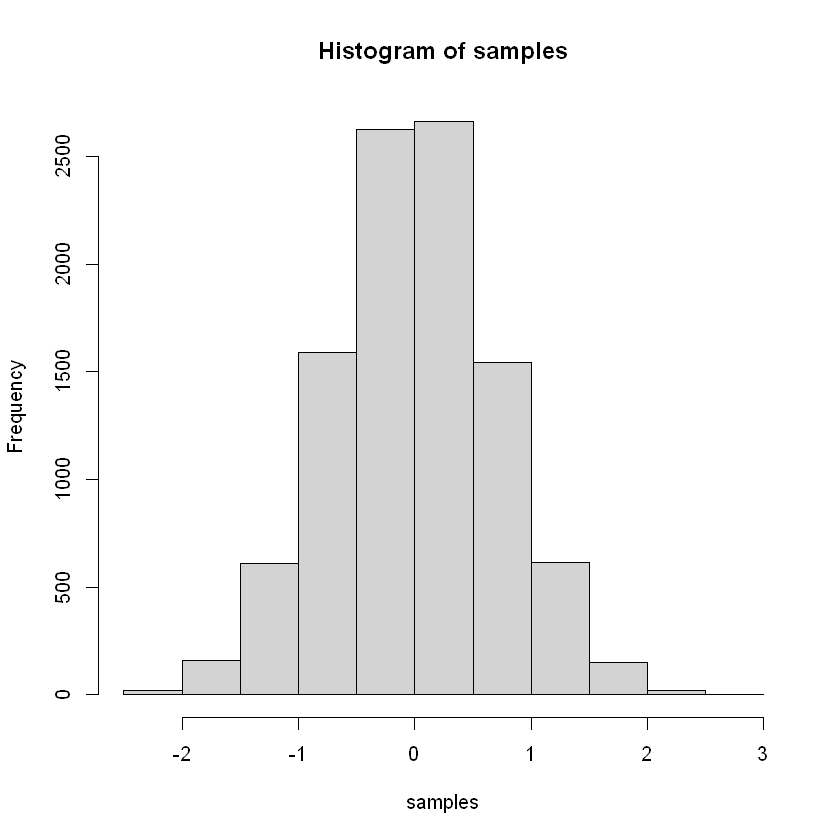
\includegraphics[width = \textwidth, height= 0.5\textheight]{hist.png}
\caption{Histogram of HMC samples}
\label{fig:hist}
\end{figure}
\end{enumerate}

 
\end{document}

